\chapter{Descrição Geral do Sistema}
%---

%---
O Software de gestão empresarial utilizado pela empresa Duas Rodas atualmente é o SAP, nele é controlado todo fluxo operacional e de funcionamento da empresa. O Agil.It trabalhará em conjunto com o SAP no módulo de manutenção de equipamentos, atuando como meio digitalizado e fazendo ponte com o SAP onde irá integrar informações prévias e competentes às ordens de manutenção.

Dividido em duas aplicações independentes, o sistema é capaz de trabalhar de forma autônoma, podendo receber e enviar dados via API ou realizar cadastros manualmente na aplicação WEB. Enquanto no aplicativo será possível acompanhar as ordens, fazer apontamentos e realizar breves consultas.

% CAP 2.1
% ---
\section{Descrição do Problema}
% ---
A gestão do processo de manutenção de máquinas é feita de forma manual. Desta forma há bastante retrabalho para repassar todos os dados ao sistema, outra preocupação é o gasto com folhas de papel. Em adendo, não há uma boa análise dos problemas comuns, equipamentos mais problemáticos, eficiência dos técnicos, entre outras.

A gestão do processo de manutenção de máquinas da empresa é feita de forma manual. Sendo assim, há bastante retrabalho por parte dos administradores e líderes do setor em questão. O tempo consumido pelos colaboradores para a correção dos problemas não permite tempo hábil para fazer a análise dos defeitos ocorridos, sendo assim existe uma dificuldade em realizar métricas desde equipamentos problemáticos até ineficiência dos técnicos.

Outra preocupação que objetiva a automatização das ordens de manutenção é o consumo excessivo de papel, pois a tendência das empresas é serem cada vez mais sustentáveis e portanto, ao digitalizar o processo de ordem de manutenção, a empresa Duas Rodas poderá  ter maiores índices de sustentabilidade e alcançar um maior destaque entre as demais empresas.
%---
% CAP 2.2

\subsection{Cenário Atual}
No processo de manutenção de equipamentos, a empresa Duas Rodas emite uma ordem de manutenção pelo SAP. Após a emissão, é impresso um formulário e entregue ao técnico elencado para a realização da manutenção. O técnico então preenche os campos básicos do formulário e depois preenche os campos que detalham as operações realizadas, bem como os componentes utilizados. Ao finalizar a manutenção, são colhidas 3 assinaturas, a do operador da máquina, a do técnico da manutenção e a do líder de manutenção, sendo que cada uma das partes pode negar a assinatura e solicitar alterações na manutenção realizada. Com todas as assinaturas rubricadas, o formulário é enviado a um funcionário administrativo que digitaliza as informações preenchidas no SAP. Além de gerar um retrabalho imenso, há um problema com a caligrafia dos manutentores, o que dificulta a digitalização dos dados. Com o volume atual de manutenções, é inviável manter o fluxo dessa forma. Com isso, entra o projeto Agil It. Atuando como meio digitalizador, faz a ponte entre a manutenção na fábrica e o sistema SAP, fazendo com que não haja mais retrabalho e eliminando totalmente os papeis utilizados nos formulários.


\begin{figure}[htb]
	\caption{\label{cenario_atual1}Cenário Atual}
	\begin{center}
		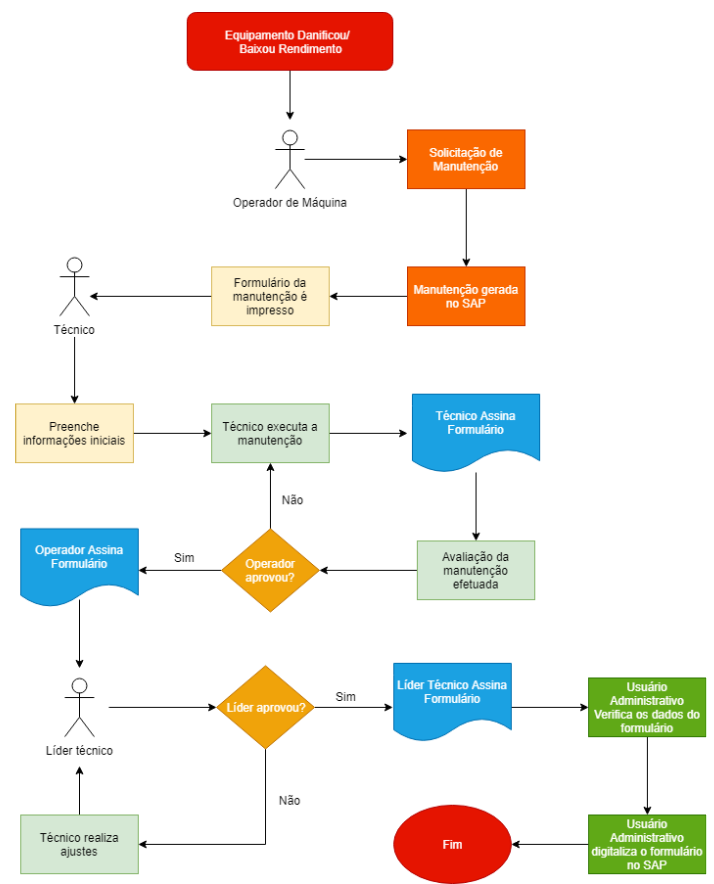
\includegraphics[scale=0.75]{./Figuras/cenario-atual1.png}
	\end{center}
	\legend{Fonte: Os Autores(2020)}
\end{figure}


\subsection{Cenário Com Agil.It}
No processo de manutenção de equipamentos com a Agil.It, a ordem de manutenção será gerada no SAP e os dados serão integrados ao sistema Agil.It. Ao ser integrado, o técnico de manutenção receberá uma notificação informando que tem uma nova OM e ele poderá visualizá-la em seu monitor no aplicativo mobile ou na aplicação WEB. Ele poderá então iniciar a manutenção e fazer os apontamentos das operações e componentes. Após finalizar a manutenção, o técnico assinará a ordem de manutenção. Após isso, o operador do equipamento será notificado e a OM ficará disponível para sua avaliação, podendo este aceitar ou recusar de acordo com as realizações do trabalho. Caso recuse, o operador deve informar o motivo da rejeição ao sistema que então, irá reabrir a OM e solicitar ao técnico para verificar. Caso o operador aceite a execução do trabalho de manutenção, o mesmo deverá assinar a OM e com isto, o sistema notificará o líder técnico, sendo o trabalho deste, averiguar a execução da tarefa, o mesmo também poderá rejeitar e solicitar alterações. Após concluído, ele deve assinar a OM. Com as 3 assinaturas colhidas, o sistema irá notificar o usuário administrador e ele poderá liberar a OM para integração com o SAP.

\begin{figure}[htb]
	\caption{\label{figure:cenario_agilit1}Cenário Agil.It}
	\begin{center}
		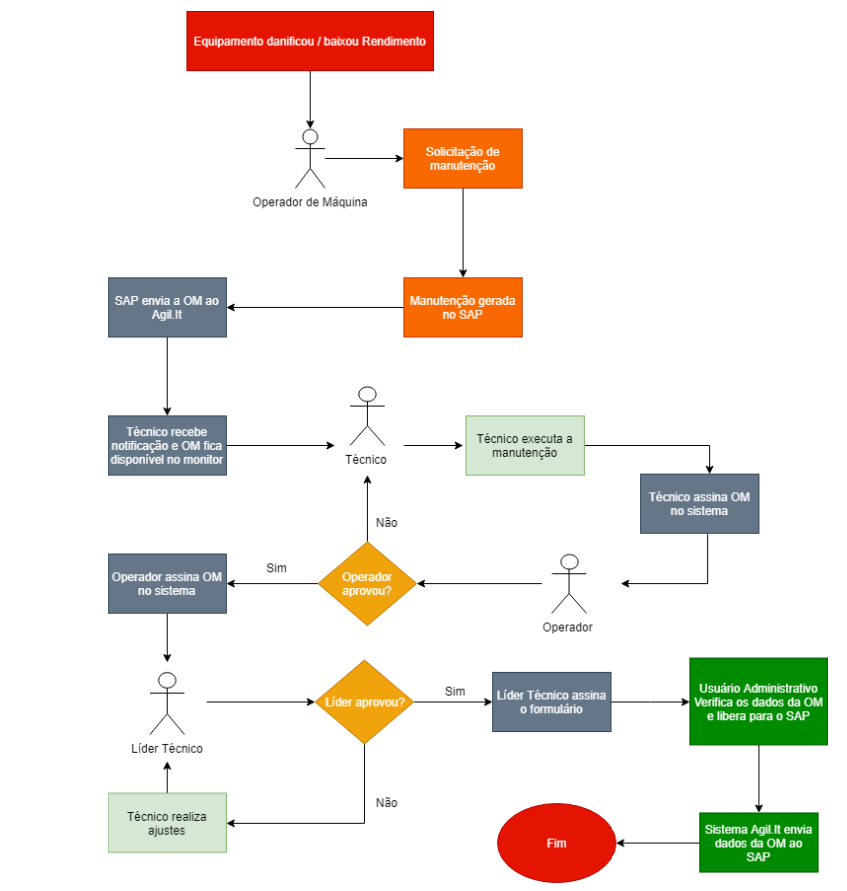
\includegraphics[scale=0.70]{./Figuras/cenario-agilit1.png}
	\end{center}
	\legend{Fonte: os autores (2020)}
\end{figure}
%---
% CAP 2.4
% ---
\section{Principais Envolvidos e suas Características}

% CAP 2.4.1
% ---
\subsection{Usuários do Sistema}
% ---
O Sistema contemplará 4 tipos de usuários, o administrador, o manutentor, o chefe de manutenção e o operário. Cada usuário terá acessos e funções diferentes no sistema. Todos terão acesso tanto a parte web da aplicação quanto a parte mobile (aplicativo).

\begin{itemize}
	
	\item O usuário administrador será responsável pelos cadastros gerais, poderá consultar e finalizar ordens de manutenção.
	
	\item O manutentor terá a visão de ordens de manutenção pendentes para ele, podendo iniciar ou pausar alguma a qualquer momento. Depois de finalizada, poderá realizar a assinatura da ordem.
	
	\item O chefe de manutenção receberá requisições de ordens de manutenção feitas por operadores e irá cadastra-las. Poderá distribuir as ordens aos manutentores, realizar consultas gerais e assinar as ordens.
	
	\item O operador, que poderá requisitar uma ordem de manutenção ao administrador, acompanhar as ordens solicitadas por ele e assinar a ordem após a conclusão.
	
\end{itemize}
% CAP 2.4.2
% ---
\subsection{Desenvolvedores do Sistema}
% ---
\begin{table}[htb]
	\begin{tabular}{|l|l|}
		\hline
		\textbf{Desenvolvedor} & \textbf{Atividade}    \\ \hline
		Julio                  & Aplicativo Mobile     \\ \hline
		Lucas                  & Aplicativo Web        \\ \hline
		Márcio                 & Back End / Integração \\ \hline
	\end{tabular}
\end{table}



\section{Regras de Negócio}
% ---
No contexto da Engenharia de Software as Regras de Negócios são tratadas como alguns Requisitos de Software, pois sem elas, o software não existiria. Regras de negócio são premissas e restrições aplicadas a uma operação comercial de uma empresa, que precisam ser atendidas para que o negócio funcione da maneira esperada \cite{crerie2008identificacao}.

Segundo \cite{2001SilviaInes} Regras de negócios são mais do que declarações sobre campos de dados ou implementação do sistema, elas definem tarefas dos atores da organização, os serviços que a organização dispõem e os recursos necessários para apoiar os processos do negócio.

Já \cite{1997kilovSimmonds} são mais enfáticos, para eles uma regra de negócio deve ser objetiva e definida em termos de notações matemáticas de proposições, mostrando que precisão é essencial quando formula-se as regras de negócio. Uma proposição é um fato ou estado observável de negócio envolvendo uma ou mais entidades pelo qual é possível afirmar ou negar a vericidade dessas entidades.

Desta forma as regras de Negocio da empresa de Alimentos Duas Rodas seriam:

\begin{subalineas}
	\item {Os administradores, líderes de manutenção e líderes de setor poderão criar ordens de manutenção};
	\item {Apenas o administrador poderá finalizar ordens de manutenção};
	\item {Os cadastros só serão possíveis na versão web};
	\item {Cada ordem de manutenção deve conter uma assinatura do manutentor, uma do operador ou líder de setor e uma do administrador};
	\item {Cada ordem de manutenção só pode ser finalizada após ter as 3 assinaturas};
	\item {Somente administradores terão acesso a tela de pendência de assinaturas};
	\item {Cada manutentor só pode ter uma ordem iniciada por vez};
	\item {Manutentores podem pausar ordens de manutenção};
	\item {Manutentores podem ter várias ordens pausadas ao mesmo tempo};
	\item {Pode haver mais de um manutentor por ordem de manutenção};
	\item {Uma ordem deve ter um manutentor principal};
\end{subalineas}




% ---